
\section{Dataset}
\label{section: experimental setup - dataset}




\subsection*{Frame specification}
\begin{figure}[!htb]
    \centering
    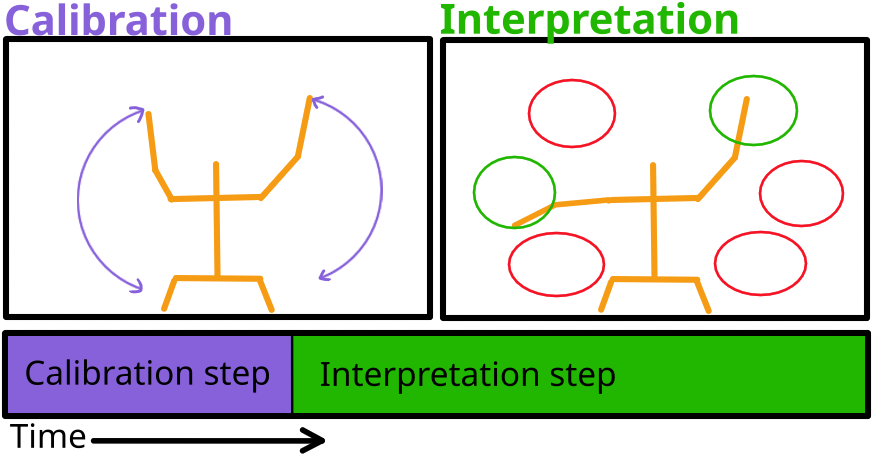
\includegraphics[width=0.7\linewidth]{figures/experimental setup/calibration vs estimation diagram.png}
    \caption{Visualisation of the two frametypes present in each recording}
    \label{fig:frame_types}
\end{figure}


% \ednote{Have an explaining asterix (*) telling why we don't use "Train/Test" as our data terms, cause this gets confusing later on with mars (As we train mars on the "IAmMuse test" data).}
% \ednote{Explain more clearly that EVERY recording has BOTH calib and usage data,}



%       -------------------------------
%     [[ Frame-by-frame data structure ]]
%       -------------------------------
% - Explain the division between "initialization frames" and "usage frames", why this is important, and how this specification is made (timestamp at MEB initialization).
% - Explain the different characteristics of these two types of frame data (initialization has both hands at the same time)
% - Mention that this "initialization" is on a \textit{recording-by-recordings} basis
% - Refer to the frame count appendix

To properly compare IAmMuse to the state-of-the-art solutions, a clear definition of the available data is required.
% We'll need a clear specification of the data that is available.
% Frame specification
First, a distinction will be made between two types of frames within any singular recording of the system.
At the start of each recording, users were instructed to calibrate the system, as is specified in \cref{sub-section: tracking method - data enhancement - minimal enclosing ball}.
Only after this calibration could the users actually use the system, since this calibration was required in order to do the data interpretation. 
We explicitly refrain from using the common machine learning terminology of \textit{training} and \textit{testing} data, for the frame types, as this would lead to confusion in \cref{section: experimental setup - baseline analysis}.
Therefore, we refer to the data used for the \textit{online few-shot training} as \textit{calibration data} and the data recording during the system usage as \textit{interpretation data}, as visualised in \cref{fig:frame_types}.

% Due to this, there are two distinct parts of each recording, where the user acts very differently in each, a visualisation of which is visible in \cref{fig:frame_types}.
% % init data
% Firstly, we have the \textbf{calibration data}, the data recorded during the \textit{online few-shot learning}.
% At this stage, the user moved their hands up and down at a steady pace.
% % prior to the user being told that the initialisation is complete, where the user moved both hands up and down at a steady pace.

Each recording contains \textbf{both} \textit{calibration data} and \textit{interpretation data} as the user recalibrates the system at the start of each recording.
The distinction between the two types of data is critical due to the unique user behaviour in each step.
In the calibration step, the user moves both their hands up and down at a steady rate.
Conversely, in the interpretation step, the user intermittently moves their arms to specific positions and holds that static pose.
% \ednote{also provide this in actual time, or make sure you do that earlier}
Each recording has an average of $212$ \textit{calibration frames} and $1184$ \textit{interpretation frames}, resulting in an average duration of 140 seconds.
The exact numbers for each recording can be found in Appendix~\ref{appendix: recording frame distribution}.



% % usage data
% Data recorded after the brief learning stage is called the \textbf{usage data} and is what is \textit{evaluated} by IAmMuse.
% % After the initialisation data, there is also the \textbf{usage data}, all data, from the moment the user was told that the system was initialised. 
% In this data, the user moves their hands to specific zones and holds them there for a certain amount of time to generate a note.
% It is crucial to make a distinction between these two types of data since the user behaviour is inherently different between the two steps. 
% Any comparison between IAmMuse and other systems needs to consider the evaluation results of specifically the \textit{usage data} for both systems, since IAmMuse does not evaluate the \textit{calibration data}.
% % The separation between \textit{calibration data} and \textit{usage data} is the moment when the calibration has completed.
% The exact number of frames of \textit{calibration data} and \textit{usage data} for each recording can be found in Appendix \ref{appendix: recording frame distribution}.



\subsection*{Recording types}

%         ---------------------------
%       [[ Different recording types ]]
%         ---------------------------
% - Describe the two types of recordings which exist, \textbf{standard} and \textbf{free play}.
% - Specify that this is \textbf{only} applicable to the \textit{usage frames} and that the type of initialisation is the same.
% - Explain why this choice for standardised was made (comparability over recordings)
% - Explain why the choice for free play was made (more realistic system usage data)
% - Refer to the standardised movement set appendix

The recordings are also split into two distinct groups, where the user follows different instructions.
% The user follows different instructions for each recording type, though the calibration stays the same.
The \textit{calibration data} of these recordings will be very similar, as the two types of recording require the same type of calibration.
The \textit{interpretation data}, however,  will vary based on the recording type.
% Therefore, the \textit{usage data} will vary in characteristics depending on the recording type.
% The difference between these two types of recordings is how the user acted during the usage of the system; thus, the only significant difference is in the way the \textit{usage data} looks.
% Standard
Firstly, there is the \textbf{standard recording}, in which the researcher instructed the user on how they should move, in accordance with a script, which can be found in Appendix \ref{appendix: standardised movement set}.
In this standardised script, the users hold various arm positions for 2-3~seconds.
% The users were to hold each position for 2-3 seconds. 
The script was designed to be simple to follow for the user by following a logical pattern while also covering every transition between distinct arm poses.
These standard recordings were designed to provide a clear comparison between users and also to provide a stable training set for any Deep Learning models.
For most users, there are \textit{three recordings} of the standardised user set.
However, due to data corruption, two users only have \textit{two standard recordings}.
%for two users, one of these three recordings got corrupted, thus they only have two.

% Free play
The second type of recording is called a \textbf{free play} recording.
% These recordings should be a good representation of how users would use the system in real-life circumstances.
These recordings simulate a realistic usage scenario, offering a more accurate representation of the input data IAmMuse is expected to process.
% These recordings are a fair representation of how users would use a system such as IAmMuse in a realistic scenario.
These recordings were made after the standard recordings, to ensure some familiarity with the system.
The users were instructed to freely explore the musical interface, leading to more realistic behaviour patterns while they tried to make their own music.
% The only input the users got at this stage was to "use the system for fun"; this led to the users exploring the system freely, trying to see what they could do, or even trying to make their own music.
Different users made a different number of free-play recordings, due to the more open-ended nature of this recording type.
% as they wanted to experiment with the system for a different amount of time.



%         -----------------
%       [[ Different users ]]
%         -----------------
% - Discuss the different users, the number we had, and the variations in them.
% - Specify that \textit{a few recordings} got \textbf{corrupted} (failed to save, for one reason or another)
% - Specify that different users made a different number of \textit{free play} recordings



%         -----------------------
%       [[ Recap and terminology ]]
%         -----------------------
% - Small recap, quickly describing the different terms used, such as the \textit{types of frames}, \textit{types of recording}, etc

% Explain what data was collected, 

% define some common terms used throughout other parts of the dataset and evaluation parts (two types of recordings, initialization data, evaluation data, etc.)

